%! TEX program = lualatex

\documentclass[nobackground,dvipsnames,table]{beamer}
\usepackage{tsc}
\usepackage{pdfpc}
\usepackage{pgfpages}
\usepackage{multimedia}

\mode<presentation>
{\usetheme{default}
	\usecolortheme{tsc}
	\setbeamercovered{transparent}
	\useinnertheme[shadow=false]{rounded}
	\usebackgroundtemplate{}
	\setbeamercolor*{frametitle}{parent=palette primary}
	\setbeamerfont{block title}{size={}}
	\setbeamertemplate{navigation symbols}{}
    \setbeamertemplate{itemize items}[circle]
}


\title[Introduction to Trust \& Safety]{Introduction to Trust \& Safety}
%\subtitle{A document made with thought and care}

\author[François and Rosenblat]{Camille François (Columbia University / Niantic Labs) Mariana Olaizola Rosenblat (NYU Stern Center for Business and Human Rights)}
%\institute[TSC]{\large Trust \& Safety Teaching Consortium}
\date[2023]{}
\subject{Trust and Safety}

\AddToShipoutPictureBG*{
  \AtPageLowerLeft{\hspace{-0.4cm}
    
\includegraphics[width=13.1cm]{img/consortium-image}}
}
% Change this to make a file with just slides, just notes or both
%\setbeameroption{hide notes}                 % Only slides
%\setbeameroption{show only notes}            % Only notes
\setbeameroption{show notes on second screen} % Both

\begin{document}

%\coverpage

\begin{frame}
	\titlepage
\end{frame}


\section{Introduction}

\begin{frame}{Learning objectives}
	Today we will:
	\begin{itemize}
		\item Learn about the purpose and history of trust \& safety
		\item Learn about approaches to trust \& safety
	\end{itemize}
\end{frame}

\section{Purpose and history of trust \& safety}


\begin{frame}{What drives trust \& safety?}
	\begin{itemize}
		\item Corporate responsibility
		\item Crisis sensitivity (cf. Zoom paper)
		\item Regulation, regulatory pressure (from Europe's DSA to the Australian Safety by Design framework)
		\item Upstream technological standards applied through the stack (see, e.g., Apple’s app rules)
		      \note[item]{"Trust and safety is the study of how people abuse the internet to cause real human harm, often using [online] products the way they are designed to work" (Journal of Online Trust \& Safety).}
		      \note[item] {Trust and Safety is also a practice and a field within technology companies that is concerned with the reduction, prevention, and mitigation of online harms. Per the Trust \& Safety Professional Association: "As internet communities, online services, and the use of digital technologies to mediate our  daily lives and interactions have continued to grow, technology companies have needed to determine the kinds of content and behaviors that are appropriate and those that are not. The teams that handle this responsibility often fall under the general term 'trust and safety.'" Source: App store review guidelines, \url{https://developer.apple.com/app-store/review/guidelines/}}
	\end{itemize}
\end{frame}


\begin{frame}{High-level taxonomy of relevant abuses}
	Violent \& Criminal Behavior
	\begin{itemize}
		\item Dangerous Organizations (e.g., extremist groups, criminal organizations)
		\item Violence (e.g., explicit threats, bomb-making instructions)
		\item Child Abuse \& Nudity (e.g., child sexual abuse material, solicitation of minors)
		\item Sexual Exploitation (e.g., non-consensual sex acts, sextortion)
		\item Human Exploitation (e.g., human trafficking, forced marriage)
		      \note[item]{Adapted from TSPA page on "Abuse Types" in T\&S: \url{https://www.tspa.org/curriculum/ts-fundamentals/policy/abuse-types/} Summarized by ChatGPT}
	\end{itemize}
\end{frame}


\begin{frame}{High-level taxonomy of relevant abuses}
	Regulated Goods \& Services
	\begin{itemize}
		\item Regulated Goods (e.g., weapons, drugs, alcohol, endangered animals)
		\item Regulated Services (e.g., gambling, addiction treatment, financial services)
		\item Commercial Sexual Activity (e.g., advertisements for sex work, selling access to nude images)
		      \note[item]{Adapted from TSPA page on "Abuse Types" in T\&S: \url{https://www.tspa.org/curriculum/ts-fundamentals/policy/abuse-types/} Summarized by ChatGPT}
	\end{itemize}
\end{frame}

\begin{frame}{High-level taxonomy of relevant abuses}
	Offensive \& Objectionable Content
	\begin{itemize}
		\item Hateful Content (e.g., slurs, support for supremacy movements, mockery of victims)
		\item Graphic \& Violent Content (e.g., imagery of fatal incidents, dismembered bodies, animal cruelty)
		\item Nudity \& Sexual Activity (e.g., pornography, explicit art)
		      \note[item]{Adapted from TSPA page on "Abuse Types" in T\&S: \url{https://www.tspa.org/curriculum/ts-fundamentals/policy/abuse-types/} Summarized by ChatGPT}
	\end{itemize}
\end{frame}

\begin{frame}{High-level taxonomy of relevant abuses}
	User Safety
	\begin{itemize}
		\item Suicide \& Self Harm (e.g., intention to self harm, encouraging self harm, instructions)
		\item Harassment \& Bullying (e.g., hateful conduct, dogpiling, blackmail threats, doxxing)
		\item Dangerous Misinformation \& Endangerment (e.g., conspiracy theories, false safety info, dangerous challenges)
		      \note[item]{Adapted from TSPA page on "Abuse Types" in T\&S: \url{https://www.tspa.org/curriculum/ts-fundamentals/policy/abuse-types/} Summarized by ChatGPT}
	\end{itemize}
\end{frame}

\begin{frame}{High-level taxonomy of relevant abuses}
	Scaled Abuse
	\begin{itemize}
		\item Spam (e.g., mass unsolicited messaging, auto-generated comments)
		\item Malware (e.g., viruses, spyware, ransomware)
		\item Inauthentic Behavior (e.g., fake engagement, disinformation campaigns)
		      \note[item]{Adapted from TSPA page on "Abuse Types" in T\&S: \url{https://www.tspa.org/curriculum/ts-fundamentals/policy/abuse-types/} Summarized by ChatGPT}
	\end{itemize}
\end{frame}

\begin{frame}{High-level taxonomy of relevant abuses}
	Deceptive \& Fraudulent Behavior
	\begin{itemize}
		\item Fraud (e.g., loan scams, pyramid schemes, fake charity solicitation, stolen goods)
		\item Impersonation (e.g., hacked accounts, fake names, impersonating celebrities)
		\item Cybersecurity (e.g., phishing, sharing/requesting login details)
		\item Intellectual Property (e.g., unauthorized use of trademarks/copyrighted content)
		\item Defamation (e.g., publication of false or outdated damaging statements)
		      \note[item]{Adapted from TSPA page on "Abuse Types" in T\&S: \url{https://www.tspa.org/curriculum/ts-fundamentals/policy/abuse-types/} Summarized by ChatGPT}
	\end{itemize}
\end{frame}

\begin{frame}{High-level taxonomy of relevant abuses}
	Community-Specific Rules
	\begin{itemize}
		\item Format (e.g., word limits, restrictions on links, insufficient details)
		\item Content Limitation (e.g., off-topic content, selling/advertising restrictions, spoilers)
		      \note[item]{Adapted from TSPA page on "Abuse Types" in T\&S: \url{https://www.tspa.org/curriculum/ts-fundamentals/policy/abuse-types/} Summarized by ChatGPT}
	\end{itemize}
\end{frame}

\begin{frame}{High-level taxonomy of relevant abuses}
	Key point: Relevant abuse types depend on your audiences, feature, product, etc.
	\note[item]{Adapted from TSPA page on "Abuse Types" in T\&S: \url{https://www.tspa.org/curriculum/ts-fundamentals/policy/abuse-types/} Summarized by ChatGPT}
\end{frame}

\begin{frame}{History and evaluation of T\&S field}
	\footnotesize
	Origins
	\begin{itemize}
		\item Ebay: prominent early user of term "trust \& safety"
	\end{itemize}
	Where T\&S "grew" from:
	\begin{itemize}
		\item Operations (ex. eBay: from Customer Service)
		\item Legal (ex. "Origins of Trust \& Safety" Databite podcast with Alexander MacGilivray and Nicole Wong)
		\item Information Security, Cybersecurity (ex: Alex Stamos "Battle for the Soul of the Internet" lecture)
	\end{itemize}
	Expanding scope of T\&S
	\begin{itemize}
		\item Today, Trust \& Safety teams across industry have different scopes, missions and organizational structures: the field continues to evolve.
	\end{itemize}
	As an academic topic, T\&S  shares borders with:
	\begin{itemize}
		\item Internet governance, cybersecurity, Internet Policy,  Internet freedom, platform governance, but also online terrorism and violent extremism, disinformation, hate speech, online forensics, etc.
	\end{itemize}
	\note[item]{Cryst, E., Grossman, S., Hancock, J., Stamos, A., \& Thiel, D. (2021). Introducing the Journal of Online Trust and Safety. Journal of Online Trust and Safety, 1(1). Retrieved from \url{https://tsjournal.org/index.php/jots/article/view/8}}
\end{frame}

\section{Approaches and best practices in T\&S}



\begin{frame}{Reactive vs. proactive models}
	\begin{columns}
		\begin{column}{0.5\textwidth}  %%<--- here
			Reactive moderation
			\begin{itemize}
				\item Responding to user reports
				\item Automatically flagging content
			\end{itemize}
			Proactive approaches
			\begin{itemize}
				\item Safety by design
			\end{itemize}
		\end{column}
		\begin{column}{0.5\textwidth}
			\begin{center}
				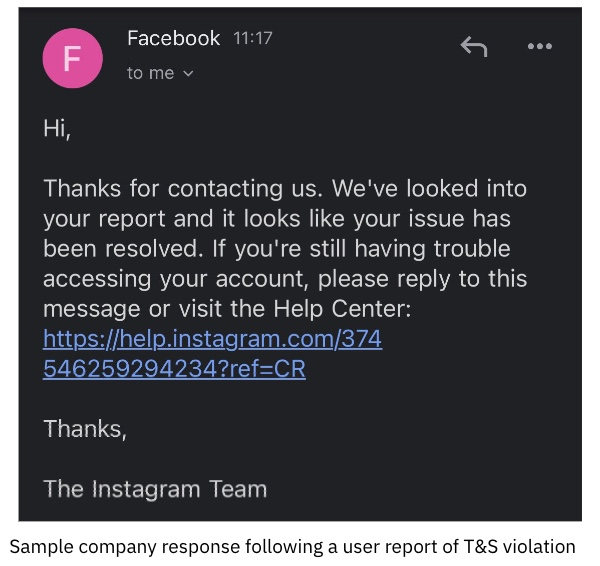
\includegraphics[width=0.9\textwidth]{img/response.jpg}
			\end{center}
		\end{column}
	\end{columns}
\end{frame}

\begin{frame}{Managing trade-offs}
	\begin{itemize}
		\item Privacy and safety may sometimes be at odds
		\item Restrictive platform features that require less moderation v. open features that require more moderation
		\item More false positives or more false negatives
	\end{itemize}
\end{frame}

\section{Where T\&S fits in an organization}

\begin{frame}{Gaining senior management support}
	\begin{itemize}
		\item Educating senior management about issues
		\item Making the case for why trust \& safety is related to core product mission
		\item Involving senior management in important edge case decisions
	\end{itemize}
\end{frame}

\begin{frame}{Building a T\&S team}
	\begin{columns}
		\begin{column}{0.5\textwidth}  %%<--- here
			Reactive moderation
			\begin{itemize}
				\item Components of a T\&S team
				\item Types of T\&S teams
				\item Types of T\&S professionals
			\end{itemize}
		\end{column}
		\begin{column}{0.5\textwidth}
			\begin{center}
				
\includegraphics[width=0.9\textwidth]{img/puzzle.jpg}
			\end{center}
		\end{column}
	\end{columns}
\end{frame}

\begin{frame}{Sample functions}
	\begin{figure}[ht]
		\begin{center}
			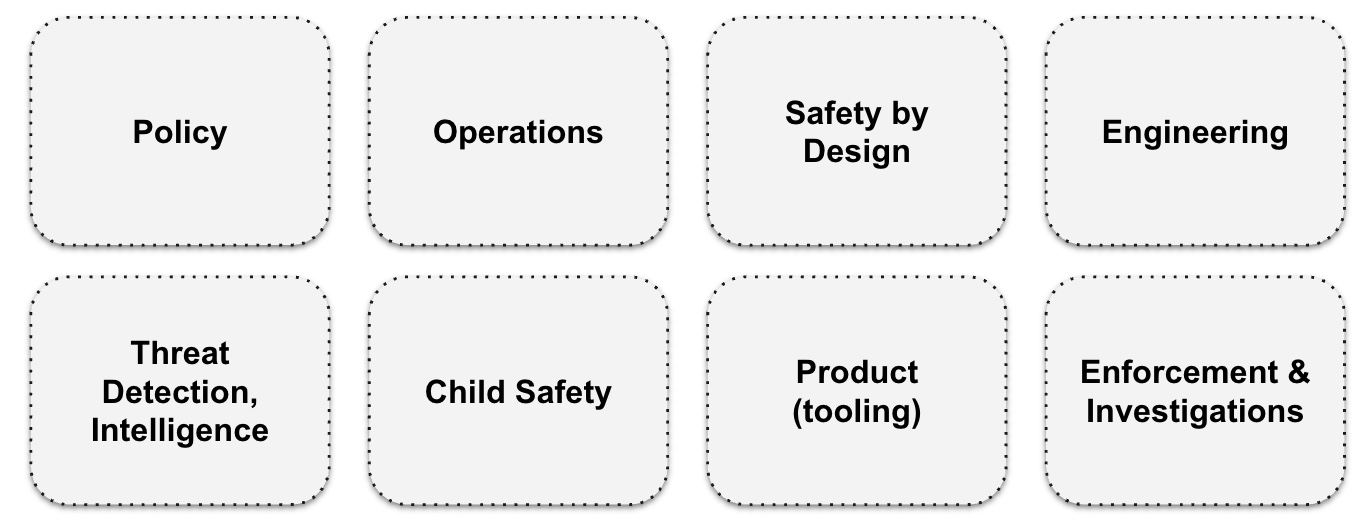
\includegraphics[width=0.9\textwidth]{img/squares.jpg}
		\end{center}
	\end{figure}
\end{frame}

\begin{frame}{Discussion: Contrasting perspectives on building T\&S teams}
	\begin{itemize}
		\item What resonated from the stories collected and shared by Alex Feerst?
		\item What are themes echoed by Feerst, by Zoom and Pinterests’ papers, and by Nicole Wong + Alexander MacGilivray?
		\item What are significant differences emerging from these testimonies?
	\end{itemize}
\end{frame}

\section{Technologies used to implement T\&S}

\begin{frame}{Overview of automated technologies}
	\begin{itemize}
		\item Digital hash technology
		\item Image recognition tools
		\item Metadata filtering
		\item Natural language processing (NLP) classifiers
		      \note[item]{"These tools can be deployed across a range of categories of content and media formats, as well as at different stages of the content lifecycle, to identify, sort, and remove content."
			      Source: {\tiny https://www.newamerica.org/oti/reports/everything-moderation-analysis-how-internet-platforms-are-using-artificial-intelligence-moderate-user-generated-content/how-automated-tools-are-used-in-the-content-moderation-process/}}
	\end{itemize}
\end{frame}

%\backpage

\end{document}